\chapter{Technical Background}
\label{chapter:background}

\begin{quote}
{\itshape
This chapter presents the concepts related to the creation of malware ground truth.

This first section introduces the development process of Android applications and the techniques used to guarantee the security and the privacy of Android users.

The second section explains the components of malware ground truth and the information gathered by the security community to support their creation.

The third section gives an overview of the construction of machine learning systems built to detect malicious applications from malware ground truth.
}
\end{quote}

\localtableofcontents{}

\section{Android ecosystem}
\subsection{Overview}
The first stable version of Android was released on the 23rd of September 2008 by Google LLC and members of the Open Handset Alliance~\cite{android_developers_announcing_2008}.
The core technologies of the system are written mainly in C and C++ while the graphical interface and the software development kit are developed with Java~\cite{open_hub_android_2019}.
Android is based on a modified version of the Linux kernel and licensed under the Apache License 2.0~\cite{android_android_2019-1}.
As a consequence, components of the Android project are accessible under a permissive open source license that allows researchers and other experts to analyze the source code and understand the internal structure of the project. 

\begin{figure}[!ht]
        \centering
	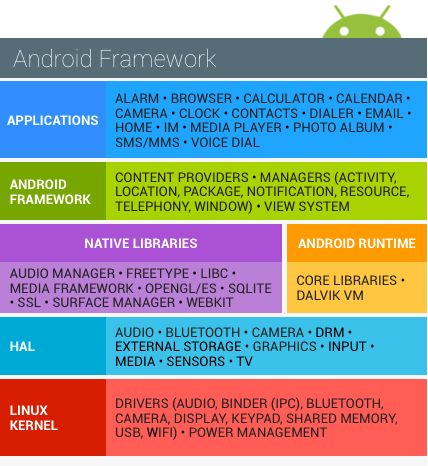
\includegraphics[width=0.6\linewidth]{figures/background/framework.png}
        \caption[Elements of the Android framework]{Components of the Android framework, Android Source~\cite{android_source_android_nodate}}
	\label{figure:background:framework}
\end{figure}

The software development kit of Android provides several services to mobile developers.
Figure~\ref{figure:background:framework} enumerates the components that are part of the Android framework proposed by Google LLC.
At the bottom of the diagram, we find the Linux Kernel and the HAL services that implement the interface between the hardware and the software stack.
The middle part of the diagram lists the native libraries, the runtime and the components of the framework that are installed to support the creation of Android applications.
Finally, the top of the diagram gives some examples of applications that are pre-installed on Android devices, such as Internet browsers, media players and calculators.

Official and third-party application stores support the distribution of Android applications.
Google Play (previously known as Android Market) is the official application store created by Google LLC on the 22nd of October 2008 to download Android applications and other digital media such as music, books, and movies~\cite{google_google_2019}.
On the one hand, mobile developers can publish their applications on Google store and add promotional contents like videos, graphics or descriptions.
On the other and, Android users can use Google Play to find more applications, install them on their devices and comment or rate the applications in order to share their experience with other users.
Google Play also features a developer policy center~\cite{android_developer_2019} and application security systems~\cite{google_google_2019-1} to guarantee the security and the privacy of Android users.
\subsection{Applications}
An Android application is a file that can be installed on Android devices to propose new services.
For instance, Android users can install applications from Google Play~\cite{google_google_2019} to read books, monitor their glucose levels or send short messages to their friends.
While Android applications are isolated from each other thanks to the Android sandbox system~\cite{android_developers_application_2019}, developers can leverage the inter-process communication mechanisms provided by intents~\cite{android_developers_intents_2019} to communicate messages across applications installed on the same device.
Thus, software components such as activities that display maps or sends rich content can be reused to improve the experience of Android users.

From a technical point of view, an Android application is a zip archive whose file name ends with the extension '.apk'.
Similar to zip archives, the content of Android applications can be extracted with standard tools to retrieve their content without information loss.
The following list shows the structure of most Android applications.

\begin{itemize}
  \item \textbf{classes.dex}: A packaged and compiled version of the application source code.
  \item \textbf{resources.arsc}: A file that indexes simple values like string translation or layout configurations.
  \item \textbf{META-INF/}: A folder used to certify the origin of the application and the integrity of files in the archive.
  \item \textbf{lib/}: A folder that provides native libraries to access the physical components of the device directly from the application.
  \item \textbf{res/}: A folder that contains additional files to support the application, such as images or audio files.
  \item \textbf{assets/}: An alternative folder to provide additional files where resource identifiers are not linked at compile time.
  \item \textbf{AndroidManifest.xml}: A file that enumerates essential information about the application, such as the package name, the version number or the software and hardware features that the application requires.
\end{itemize}

\begin{table}[!ht]
\centering
  \label{table:background:versions}
  \caption[History of Android versions]{History of Android versions~\cite{android_android_2019}}
  \begin{tabular}{| c | r |  r | r | r |}
    \hline
    \textbf{Name}      & \textbf{Version} & \textbf{Release}   & \textbf{API} \\ \hline
    (no codename)      & 1.0              & September 23, 2008 & 1 \\ \hline
    Petit Four         & 1.1              & February 9, 2009   & 2 \\ \hline
    Cupcake            & 1.5              & April 27, 2009     & 3 \\ \hline
    Donut              & 1.6              & September 15, 2009 & 4 \\ \hline
    Eclair             & 2.0 - 2.1        & October 26, 2009   & 5 - 7 \\ \hline
    Froyo              & 2.2 - 2.2.3      & May 20, 2010       & 8 \\ \hline
    Gingerbread        & 2.3 - 2.3.7      & December 6, 2010   & 9 - 10 \\ \hline
    Honeycomb          & 3.0 - 3.2.6      & February 22, 2011  & 11 - 13 \\ \hline
    Ice Cream Sandwich & 4.0 - 4.0.4      & October 18, 2011   & 14 - 15 \\ \hline
    Jelly Bean         & 4.1 - 4.3.1      & July 9, 2012       & 16 - 18 \\ \hline
    KitKat             & 4.4 - 4.4.4      & October 31, 2013   & 19 - 20 \\ \hline
    Lollipop           & 5.0 - 5.1.1      & November 12, 2014  & 21 - 22 \\ \hline
    Marshmallow        & 6.0 - 6.0.1      & October 5, 2015    & 23 \\ \hline
    Nougat             & 7.0 - 7.1.2      & August 22, 2016    & 24 - 25 \\ \hline
    Oreo               & 8.0 - 8.1        & August 21, 2017    & 26 - 27 \\ \hline
    Pie                & 9.0              & August 6, 2018     & 28 \\ \hline
    Android Q          & 10.0             &                    & 29 \\
    \hline
  \end{tabular}
\end{table}


As new versions of the Android project are released over time, external applications must maintain a level of backward compatibility to support the execution environments deployed on user devices.
Table~\ref{table:background:versions} details the versions of Android published by Google LLC starting from version 1.0.
Each release is associated with a code name, a version number and an API level targeted by application developers to indicate the degree of compatibility that the application ensures.
For instance, an application with a minimum API level of 23 will be compatible with Android devices that feature an API level greater or equals to 23.
This information can be found in the 'AndroidManifest.xml' file of the application.
\subsection{Security model}

\begin{figure}[!ht]
        \centering
	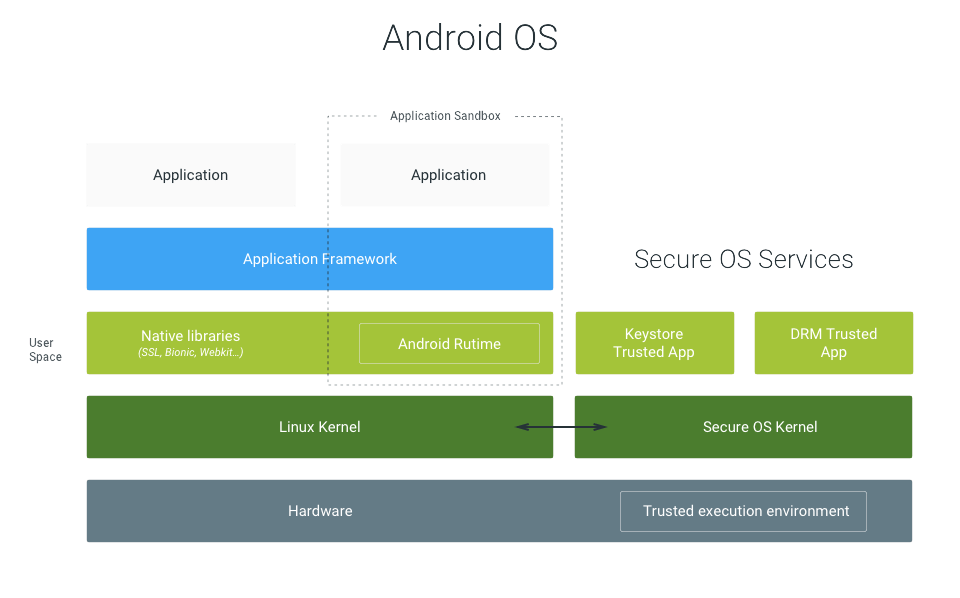
\includegraphics[width=\linewidth]{figures/background/security.png}
        \caption[Components related to Android security]{Components of Android security, Android Website~\cite{android_website_android_2019}}
	\label{figure:background:security}
\end{figure}

First and foremost, the security of Android applications depends on the integrity of the layers that support their execution.
Figure~\ref{figure:background:security} shows the parts of the Android framework that are responsible for the security of Android applications as described on the Android developers' website~\cite{android_website_android_2019}.
Similar to Figure~\ref{figure:background:framework}, the hardware and the operating system layers powered by the Linux kernel are run in a trusted execution environment to ensure the security of the underlying system.
Then, the Android framework implements several trusted services in user space such as keystore and DRM to enable the creation of secure applications.
Finally, applications are executed in a sandbox system that isolates their runtime context from the rest of the system, including access from other applications.

\begin{figure}[!ht]
        \centering
	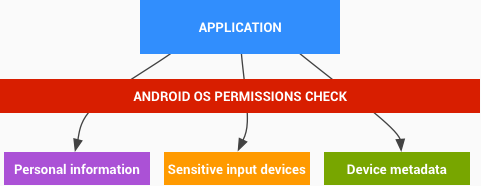
\includegraphics[width=0.75\linewidth]{figures/background/permissions.png}
        \caption[Android relies on permission checks to protect private data]{Android relies on permission checks to protect private data, Android Website~\cite{android_developers_application_2019-1}}
	\label{figure:background:permissions}
\end{figure}

Several features are also implemented to secure Android at the application level~\cite{android_developers_application_2019-1}.
By default, Android applications can not access the most critical system resources such as camera functions, network connections, and location data as a result of the application sandbox.
Figure~\ref{figure:background:permissions} illustrates that the Android permission model ensures that applications can access personal information or device metadata only with the consent of the device owner.
This verification process extends to cost-sensitive resources such as billing services or SIM card accesses.
Android applications must also be signed before their distribution on application stores to identify application authors and make them accountable for the potential misbehavior of their application.
In addition to technical implementations, the Android developers' website proposes several education resources to encourage the best development practices~\cite{android_developers_security_2019}.

In 2017, Google LLC announced the released of Google Play Protect~\cite{tetali_keeping_2018}, a machine learning based system that detects malicious applications on user devices.
Google Play Protect continuously scans applications to find harmful behaviors and submit them to security experts for an extensive review.
Malicious applications are then grouped into families to uncover similar applications that are not yet recognized by the security system.
The same year, the Google security team announced that their machine learning based system detected 60.3\% of malware identified by Google Play Protect to further secure Android devices~\cite{tetali_keeping_2018}.
\section{Malware ground truth}
\subsection{Files}
A ground truth of Android malware is a collection of Android applications that are recognized as either malicious or harmful for a security expert.
The main goal of malware ground truths is to provide reference datasets that researchers and other security experts can use in their experiments to design better security solutions.
These datasets are important for the scientific community, as they allow research groups to engage in reproducible experiments which guarantees the quality of their research output.
Moreover, malware ground truths are crucial to the performance of machine learning algorithms, as the training and the results of these algorithms depends on the quality of the samples used as examples~\cite{rossow_prudent_2012,sommer_outside_2010}.

\begin{table}[!ht]
\centering
  \label{table:background:markets}
  \caption[Distribution of Android applications by markets on Androzoo]{Distribution of Android applications by markets on Androzoo~\cite{allix_androzoo:_2016}}
  \begin{tabular}{| l | r |}
    \hline
    \textbf{Market} & \textbf{Count} \\ \hline
    play.google.com & 7,048,293 \\ \hline
    anzhi           & 832,997 \\ \hline
    appchina        & 771,970 \\ \hline
    mi.com          & 113,583 \\ \hline
    1mobile         & 57,530 \\ \hline
    angeeks         & 55,818 \\ \hline
    slideme         & 52,467 \\ \hline
    fdroid          & 18,304 \\ \hline
    praguard        & 10,186 \\ \hline
    torrents        & 5,294 \\ \hline
    freewarelovers  & 4,145 \\ \hline
    proandroid      & 3,683 \\ \hline
    hiapk           & 2,512 \\ \hline
    genome          & 1,247 \\ \hline
    apk\_bang        & 363 \\ \hline
    unknown         & 138 \\
    \hline
  \end{tabular}
\end{table}


To illustrate the definition of malware ground truths, we will consider the case of the Androzoo project created by the University of Luxembourg.
Androzoo is a collection of Android applications gathered from a broad set of application stores.
Table~\ref{table:background:markets} shows the distribution of applications by Android markets.
We observe that the official Android market is the main source of Android applications for the repository.
Androzoo also includes Chinese application markets such as anzhi or appchina in addition to open source applications found on the F-Droid repository.
In total, Androzoo contains more than 8 million applications as of January 2019.

One critical aspect of malware ground truths is to maintain an index that associates a unique identifier to each application in the collection.
This index is useful for security experts to aggregate multiple sources of applications or check the presence of a single application within the set.
To implement the name index, security experts rely on cryptographic hash functions that compute a fixed size string from an arbitrary size bit string, like the content of Android applications.
For instance, The SHA-256 algorithm associates a 32 bit signature to a file that can not be easily forged or inverted by an attacker.
Thus, the only feasible method to retrieve the file signature is to apply the same algorithm on the same file.
The following value is an example of SHA-256 signature formatted as an hexadecimal string and present in the Androzoo repository: '00001f58c32e40376f64cc88b70f8fad2fda054e0863abd5e41f4c6f18a65da2'.
\subsection{Metadata}
To complement the information contained in Android applications, security actors provide additional metadata to enrich the content of malware ground truth.
For instance, the Androzoo project~\cite{allix_androzoo:_2016} proposes a metadata file that details several characteristics of Android applications:

\begin{itemize}
  \item \textbf{SHA256, SHA1, MD5}: file signatures to identify the application
  \item \textbf{APK and DEX size}: size of the source code and the application
  \item \textbf{DEX date}: compilation date of the packaged source code
  \item \textbf{Market names}: markets where the application was found
  \item \textbf{Package name}: package name from the Android manifest
  \item \textbf{Version code}: version code from the Android manifest
  \item \textbf{VirusTotal detections}: number of positive detections
  \item \textbf{VirusTotal scan date}: date of the antivirus scan
\end{itemize}

This information is useful for security practitioners to search applications tailored toward a specific use case or to compute statistics about the files listed in malware ground truths.

\begin{table}[!ht]
\centering
  \label{table:background:certificate}
  \caption{Example of a developer certificate found in an Android application}
  \begin{tabular}{| l | p{12cm} |}
  \hline
  \textbf{Key}             & \textbf{Value} \\ \hline
  Owner                    &  CN=Eyvind Almqvist, OU=Mobile Visuals, O=Javsym, \newline L=Kista, ST=Kista, C=SE \\ \hline
  Issuer                   &  CN=Eyvind Almqvist, OU=Mobile Visuals, O=Javsym, L=Kista, ST=Kista, C=SE \\ \hline
  Serial number            &  4d53c582 \\ \hline
  Valid from               &  Thu Feb 10 06:01:22 EST 2011 until: Fri Jan 28 06:01:22 EST 2061 \\ \hline
  MD5                      &  58:94:63:63:C1:ED:4C:02:CE:90:CE:64:DA:D7:4A:E4 \\ \hline
  SHA1                     &  17:5C:44:E3:A6:1A:F2:4F:A5:78:6E:C7:F0:42:4C:AD:E6:F5:CA:DF \\ \hline
  Algorithm name           &  SHA1withRSA Version: 3 \\
  \hline
  \end{tabular}
\end{table}


As we mentioned in the previous section, Android applications downloaded from the official market must include a developer certificate that identifies the application authors to hold them accountable for potential misbehaviors.
The developer certificate is a public key embedded in the 'CERT.RSA' file, located in the 'META-INF' folder of the application package.
Standard cryptographic software can be used to extract this information as a human-readable text.
For instance, Table~\ref{table:background:certificate} shows an example of a developer certificate found in an Android application.
The certificate contains the owner and issuer, in addition to a serial number, an MD5, and SHA1 signature to guarantee the integrity of the certificate.
This information is essential to trace the origin of Android applications and find software packages from the same authors.

Malware ground truth can also inform about the package name and the version code of Android applications.
As multiple versions of the same application can be published, these two pieces of information help practitioners to track the lineage of Android packages over time.
On the one hand, the package name remains the same for every version of the same application and serves as a common identifier between them.
On the other hand, the version code must be different for every new version of the application to mark the evolution of the package.
Both the package name and the version code can be found in the Android manifest file.
As an example, the 'ul.edu.routes' package name can be associated both to a version '1' and a version '2' of the same application.
\subsection{Classification}
We saw that malware files and their metadata supply useful information about the content of Android applications, yet they do not inform security practitioners about the danger of malware samples.
Compared to other classification problems, Android applications require more time and expertise from specialists to decide if an application should be considered malicious or not~\cite{ics2_cybersecurity_2018}.
This limitation affects the ability of the security community to leverage malware datasets, as security experts need access to qualified classification results before they can train and evaluate new solutions.

To address this problem, the research community relies on external source information to classify Android applications at a large scale.
At least three types of techniques are available to isolate malware from the rest of Android applications:

\begin{itemize}
  \item \textbf{Internal classification}: applications are analyzed manually by a security expert to extract suspicious artifacts and establish the ground truth. This technique was applied to build the Genome dataset~\cite{zhou_dissecting_2012}.
  \item \textbf{Relative classification}: applications with similar properties are grouped into clusters where the notion of proximity depends on the definition given by the ground truth authors. This technique was used to create the Android Malware dataset~\cite{wei_deep_2017}.
  \item \textbf{External classification}: applications are analyzed by a trusted third party actor to gather classification results. This technique was involved in the creation of the Androzoo dataset~\cite{allix_androzoo:_2016} and the Drebin dataset~\cite{arp_drebin:_2014}.
\end{itemize}

Each classification method has its benefits and its drawbacks.
An internal classification scheme provides an unambiguous analysis of malware samples but at the highest cost in terms of human resources.
A relative classification scheme applies to large malware datasets, but the results of clustering algorithms are not thoroughly verified to ensure that applications are genuinely malicious.
An external classification technique is possible at a large scale and yields accurate results as long as the expertise and the availability of the third party source can be trusted.

\begin{figure}[!ht]
        \centering
	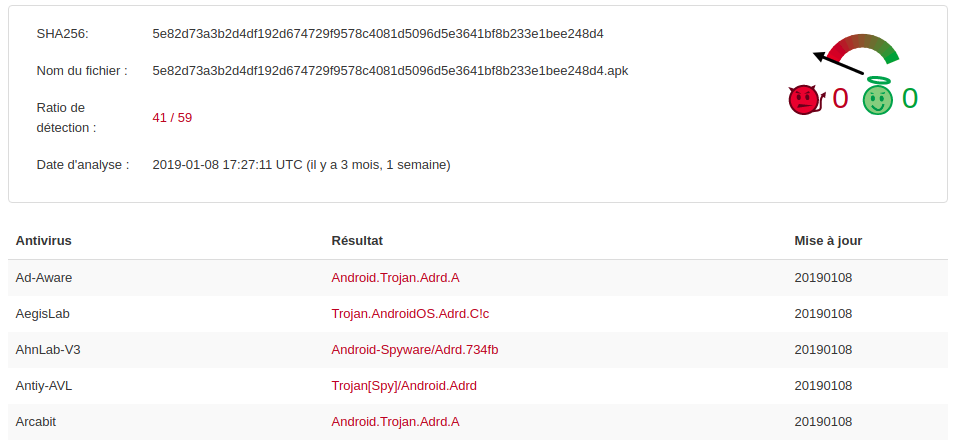
\includegraphics[width=0.9\linewidth]{figures/background/virustotal.png}
	\caption{VirusTotal report generated after the submission of an Android malware}
	\label{figure:background:virustotal}
\end{figure}

In this dissertation, we focused our work on an external classification solution built upon VirusTotal to leverage the efforts of security actors in performing malware analysis.
VirusTotal~\cite{noauthor_virustotal_nodate} is an online service that aggregates the output of commercial antivirus products to let users decide if an application should be considered malicious.
Figure~\ref{figure:background:virustotal} displays the result of a VirusTotal scan performed on an Android application.
First, a ratio of detection indicates that 41 antivirus products out of 59 consider the file as malicious.
Moreover, each antivirus that returned a positive detection supplies a label that contains several pieces of information about the malware, such as the platform, the type of threat, the name of the malware family and its variant.
While antivirus labels cannot be used as if due to their syntactic and semantic discrepancies, the information they contain can support the creation of better malware ground truth.
\section{Machine learning systems}
\subsection{Feature engineering}
The first step toward the creation of machine learning based solutions is to gather information about the task that must be learned by the algorithm and performed by the system.
For that purpose, security practitioners take advantage of existing malware ground truths as a source of examples to train and evaluate statistical models.
As information about Android applications cannot be inferred directly by algorithms, experts must engineer machine learning features that describe the task at a higher level of abstraction.
For the detection of Android malware, this step consists of analyzing Android applications to find characteristics that might support the decision of the model.

At least two types of analysis are available to mine knowledge from Android malware.
On the one hand, experts can perform static analysis to extract information about the structure of Android applications.
For instance, static analysis tools can look at the application source code, retrieve information about the resources included in the package and describe the file included in the archive.
While static analysis covers most of the information present in the application, this technique does not inform the expert about the behavior of the application at runtime.
To gather information from the execution of Android applications, practitioners turn to dynamic analysis tools for observing the actions of the application in a confined environment.
This type of analysis can find which websites the application tries to contact, which data are read or written on the device and if the application triggers on specific events (e.g.,\ the phone rebooted or connected to the Internet).
Together, static and dynamic analysis provide the raw material for the creation of machine learning features and complement each other to cover the facets of the application.

Machine learning practitioners can then engineer three types of features depending on the level of abstraction they target.
The first type is binary features that are the direct translation of the analysis results.
If an analysis reported that the application uses a particular string or a file, then this information can be converted to a simple 'yes' or 'no' structure and inform the algorithm about the presence or the absence of a particular item.
The second type is derived features that further abstract the results of the analysis.
For instance, strings found in Android applications can be scrutinized to find URL scheme or file system paths and declare that the applications might perform some file or network operations.
Finally, the third type is statistical features which are the results of a computation performed on raw data.
Statistical features provide an overview of the application characteristics, such as the number of classes it contains or the number of permissions required per line of code.
To illustrate each category, the following list provides some examples of popular machine learning features applied to the detection of Android malware:

\begin{itemize}
  \item \textbf{Binary features}: requires access to the Internet, requires a maximum API level of 19, is in debug mode, informs about the owner of the developer certificate, is vulnerable to a known CVE.
  \item \textbf{Derived features}: contains obfuscated names, performs cryptographic operations, attempts to contact a botnet URL, loads additional code at runtime, communicates with native libraries.
  \item \textbf{Statistical features}: size of the application, number of classes, number of dangerous permissions per line of code, average instructions per method, entropy of the developer certificate.
\end{itemize}

\subsection{Model training}

\begin{figure}[!ht]
        \centering
	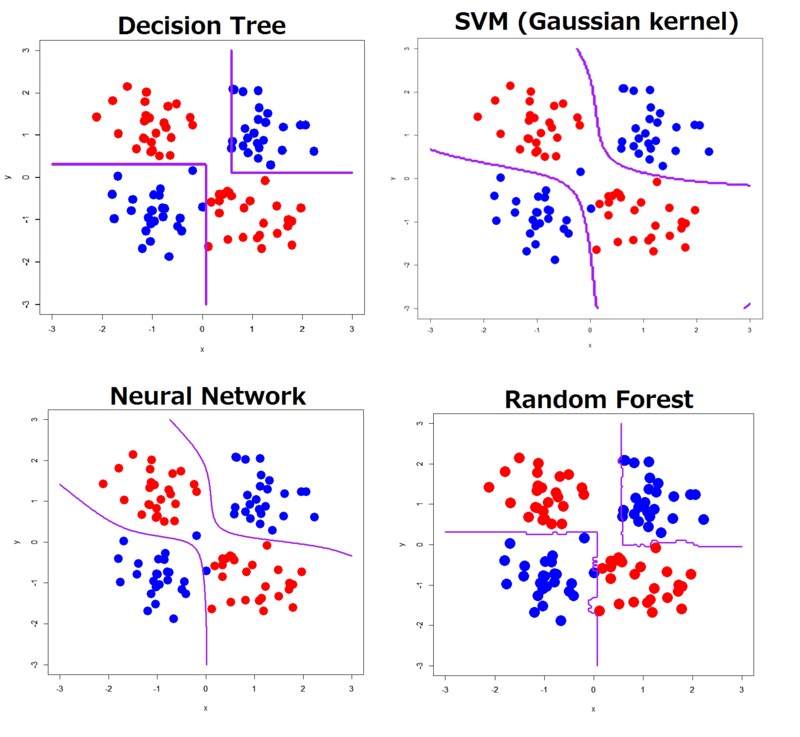
\includegraphics[width=0.75\linewidth]{figures/background/decision.png}
        \caption[Results of machine learning algorithms applied on a XOR pattern]{Example of machine learning algorithms applied on a XOR pattern~\cite{ozaki_decision_2015}}
	\label{figure:background:decision}
\end{figure}

With features engineered from ground truth datasets, machine learning algorithms can train detection models under the supervision of a security expert.
The goal of this step is to draw a decision boundary between possible outcomes, such as the possibility that an application is benign or malicious.
For instance, Figure~\ref{figure:background:decision} presents the result of four different machine algorithms in classifying a simple XOR pattern.
The decision boundary created by machine learning algorithms takes the form of a purple curve that splits the dots by colors.
During model training, the purple curves are adjusted by the algorithm to fit the data and avoid classification errors.
We can observe that different machine learning algorithms generate decision boundaries of various shapes, as the mathematical foundations of these algorithms differ.

The training process of machine learning algorithms can be explained and formalized if we consider a simple case like linear regression.
A linear regression algorithm finds a linear relationship between dependent variables and the target class.
The regression can be formulated as follow:
$$y_{i}=\beta _{0}1+\beta _{1}x_{i1}+\cdots +\beta _{p}x_{ip}+\varepsilon _{i}=\mathbf {x} _{i}^{\mathsf {T}}{\boldsymbol {\beta }}+\varepsilon _{i},\qquad i=1,\ldots ,n,$$
where $\{y_{i},\,x_{i1},\ldots ,x_{ip}\}_{i=1}^{n}$ represents an input dataset and $\beta$ the coefficients of the linear relationship.
Finding the coefficients that best fit the data can be transformed into a minimization problem where the algorithm attempts to minimize the sum of squared residuals (i.e.,\ the total difference between the actual and the predicted values):
$${\text{Find }}\min _{\beta }Q(\beta ),\quad {\text{for }}Q(\beta )=\sum _{i=1}^{n}{\widehat {\varepsilon }}_{i}^{\,2}=\sum _{i=1}^{n}(y_{i} - \beta x_{i})^{2}$$

Machine learning algorithms propose some hyper-parameters that can be tuned to limit the complexity of statistical models or prevent extreme coefficients that cause too much variance.
For instance, a linear regression algorithm can include a regularization parameter $\lambda$ that penalizes either the number of non zero coefficients (L1 norm, LASSO) or the imbalance between coefficient values (L2 norm, RIDGE).
The two approaches can also be combined to optimize both cases with a technique called Elastic Net~\cite{zou_regularization_2005}.
\subsection{Evaluation}

\begin{figure}[!ht]
  \centering
        \centering
	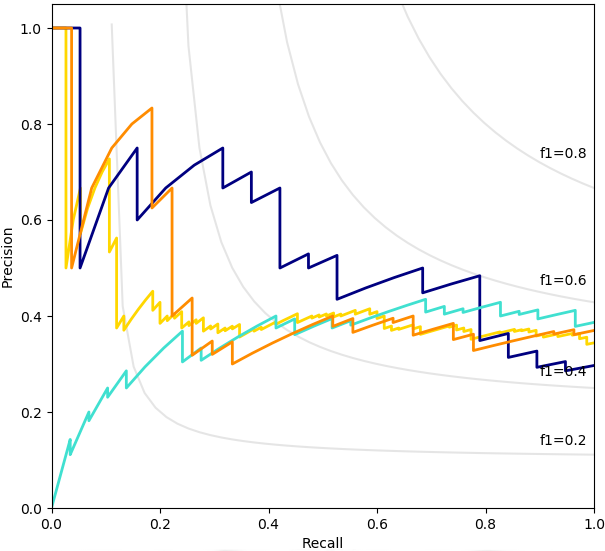
\includegraphics[width=0.6\linewidth]{figures/background/pr.png}
	\caption{Precision-Recall curve obtained from a classification problem}
	\label{figure:background:pr}
\end{figure}

As multiple choices of algorithms, coefficients, and hyper-parameters are available to train machine learning based systems, security experts must evaluate the performance of their models to explore the solutions at their disposal.
A convenient solution for practitioners is to evaluate statistical models with a set of metrics that summarizes the performances of the model on a reference dataset.
For detecting malicious Android applications, precision and recall are often used to measure the number of correct answers, depending on the type of errors.
On the one hand, the precision measures the number of correct positive results divided by the total number of positive results predicted by the algorithm:
$$precision = \frac{true\ positives}{true\ positives + false\ positives}$$
On the other hand, the recall measures the number of correct positive results divided by the total number of true results in the dataset:
$$recall = \frac{true\ positives}{true\ positives + false\ negatives}$$
The two metrics can be combined into an F1-score, which is the harmonic mean of the precision and recall that averages their values:
$$F_1 = 2 \times \frac{precision \times recall}{precision + recall}$$
In a real-world scenario, practitioners may also explore the trade-off of different models or parameters with a precision-recall curve such as Figure~\ref{figure:background:pr} to find a more suitable solution.

\begin{figure}[!ht]
        \centering
	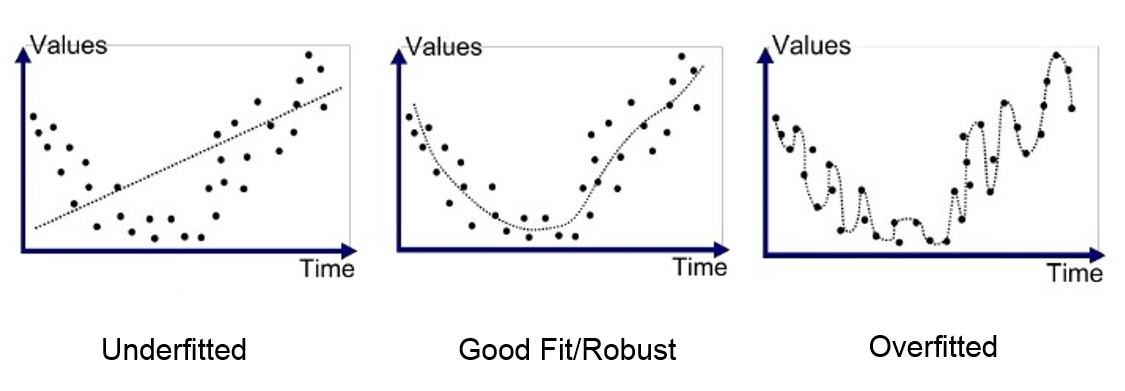
\includegraphics[width=\linewidth]{figures/background/fit.png}
        \caption[Difference between under-fitting and over-fitting]{Difference between under-fitting and over-fitting~\cite{bhande_what_2018}}
	\label{figure:background:fit}
\end{figure}

Another fundamental trade-off explored by machine learning practitioners is the ability of statistical models to store example details versus the ability to generalize on new examples.
Figure~\ref{figure:background:fit} illustrates the problem with three curves that represent the decision boundary of statistical models.
The model on the left is considered too simple (or under-fitted), as the shape of the decision boundary is linear while the data distribution is polynomial.
The model on the right is too complex (or over-fitted), since the decision boundary is too specific regarding the data provided to the algorithm.
The model in the middle offers the right balance, as the general shape of the model corresponds to the process that might generate the data points.
Best practices such as the use of cross-validation techniques and the inclusion of testing datasets can improve the robustness of machine learning experiments in practice.

In this section, we explored the use of machine learning to extract statistical patterns from a large corpus of data.
However, the task conveyed to statistical models can only be learned with a great reference ground truth that supports the training and the evaluation of machine learning algorithms.
In the absence of qualified ground truth, machine learning algorithms are at risk of proposing a model with suitable performance in the lab, but with unacceptable performance in real-world scenarios.
Thus, our comprehension of malware ground truth is crucial to the development and the adoption of machine learning based systems.
Under these circumstances, the main risk for the security community is to focus its attention only on quantitative assessments while the description of Android malware remains a vital requirement to justify the decision of automated systems.
